\subsection{Scenarios}

\begin{itemize}
    \item \textbf{Scenario 1: The Store Manager discovers the CLup System and decides to use it for his/her store.} John is the Store Manager of the main supermarket in Via Pacini, Milan. With the start of the COVID emergency and the delineation by the government of new rules on the entrances of people into the store, its store has created very long queues for 2 weeks outside the store. John realizes the danger of the situation and decides to look for a system that can regulate the entrances avoiding the creation of long queues, thus finding CLup.
    Once decided to adopt CLup for the management of queues and etrances he registers via the web app. He inserts information about him, inserts all the store information, and then decides to allow access to the system to his 5 employees: Ellen, Mike, Harry, Louis and Ricky who will handle the various phases of interaction with the system. This 5 employees are registered and will then be able to log in with their accounts as employees to the system.
    \item \textbf{Scenario 2: A User meets the CLup service and decides to give it a try.} Steve is a young guy, he lives alone in a studio apartment located in the city center of Milan. Every month he has to pay the rent, which is quite expensive, the bills and the other monthly expenses. Every week he goes to his favourite supermarket website to see what are the discounts available. While browsing the website Steve sees that the store has enabled a new service, called CLup, to reduce the physical queue present every day outside the store. 
    Every time he goes grocery shopping he loses so much time because he has to wait to get inside the store due to the limited space inside the building. He is very happy and curious about this new service. He downloads the CLup application, he opens it and decides to sign up.
    \item \textbf{Scenario 3: A User who could not reserve the seat in the queue virtually, goes to the store.} Lily is a pretty 80-year-old lady who lives with her 86-year-old husband and buys groceries every week. Unfortunately, Lily doesn’t have a smartphone and an internet connection to book a seat in the queue using CLup. Lily shows up at the supermarket and approaches the store entrance to ask if it’s possible to enter. Mike, the employee on shift at the supermarket entrance at that moment informs Lily that there is no problem and that he will be the one to reserve a queue for her.
    Mike, from his computer, makes the request to CLup web app, sees a number being generated and prints it to give it to Lily. He also informs Lily that he can wait outside the store and he will alert her when the time comes to enter.
    \item \textbf{Scenario 4: A CLup customer lines up to go grocery shopping to her favourite store.} Ester is young housewife. She has two childs, one of them is very young and he needs frequent attentions during the day. She also has to clean up the big house she lives in with her husband. Ester is very busy during the day doing such duties. She needs to go grocery shopping and she remembers that some time ago she signed up to the digital queue service CLup. She opens the application and finds that her favourite supermarket adopted the CLup system. 
    She selects the store and lines up to go shopping. While she is waiting for her turn she can play with her young son. Once arrived at the supermarket she enters the store directly showing her digital queue number.
    \item \textbf{Scenario 5: A CLup customer books a visit.} Frank opens the food storage and realizes that soon he will finish his stock of pasta. Being a lover of pasta, he knows he will have to buy more but today he has to finish working on a very important project. So Frank decides to book a visit to the supermarket in Via Pacini for tomorrow, he knows it will be short and does not want to wait in line. So Frank picks up his smartphone, opens the CLup app, enters the visits section and inserts the optional information requested by CLup. In particular, he specifies that he will go to the supermarket exclusively 
    to buy pasta and that he plans to spend a maximum of 5 minutes there. Immediately after confirming this information he slides through all available time slots in which to book his visit displayed by CLup. So he selects tomorrow at 3:30 PM. 
    \item \textbf{Scenario 6: The Store Manager views charts and statistics about entrances.} Mike is the Store Manager of a big supermarket near Porta Vittoria, situated in the metripolitan city of Milan. The Milan city council is collecting data to define the upcoming local ordinance related to the COVID-19 emergency. In particular the politicians want to know if the supermarkets are "safe" places, if they avoid creating long queues and if they are or are not overcrowded places. 
    To retrieve such informations they know that in the last month many grocery stores adopted a smart queue service called CLup. Further investigating about this innovative platform they discovered that CLup collects metrics and statistics about people entering the stores. After obtaining the necessary legal authorizations the council asks every store manager involved with CLup to report a summary of the data provided by the application. Mike logs in to the store manager administration interface, clicks on "View store charts and statistics" and reports the main informations to the city council that asked him.
    \item \textbf{Scenario 7: A CLup customer arrives late to the store and he looses his turn.} Mark is a middle-aged man working for a big tech company in Lombardia, Italy. He works in the sales and marketing repartment and he is often out of town on business. Today his driving home after a two days trip around Italy. He's stretching his legs after stopping at an auto grill and he decides to line up to go grocery shopping on the way home to see the estimated queue time. He finds that he's perfectly in time in order to go directly to the store, thus he starts driving again. 
    On the way to the store a car crash slows down his way and he arrives late to the store with respect to his turn. He tries to explain what happened to the employee checking entrances, but at end he is not allowed to enter the store because his queue number turn is expired.
\end{itemize}

\subsection{Application Domain Model}
Here is the application domain model of this project. In particular, this section focuses on the object model (\textbf{static information models} and \textbf{dynamic class behaviour models}).
\subsubsection{Static Information Model}
The below high-level diagram provides a static information model of the application domain. Basically, it is the structure of the world, it contains only few attributes, and it doesn't include every class that will be necessary to define the model of the CLup system.

The main aspects of Clup modelled in the below diagram are:
\begin{itemize}
    \item The application need to consider the presence of visitor who arrive at the supermarket and require a place in the queue. For this reason, two types of Store Clients (visitor and customer) are distinguished in the diagram
    \item Given the need to allow the reservation of a seat in the queue to those who do not use the system directly, it is necessary to distinguish between 2 types of Lineup turn (physical and virtual).
    \item A customer can book a Visit or a Lineup turn. To facilitate the reading of the diagram these two actions were generalized to an abstract class Reservation extended by Visit class and LineupTurn class. the possibility to generate a QR code associated to a reservation of a seat in queue is represented in the diagram by the optional attribute "qrCode" of the VirtualLineupTurn class
    \item A visitor can book only a physical lineup turn. This reservation is handled by a Store employee who will act as a link between the system and the visitor
    \item Each entrance could be monitored by the store manager
\end{itemize}
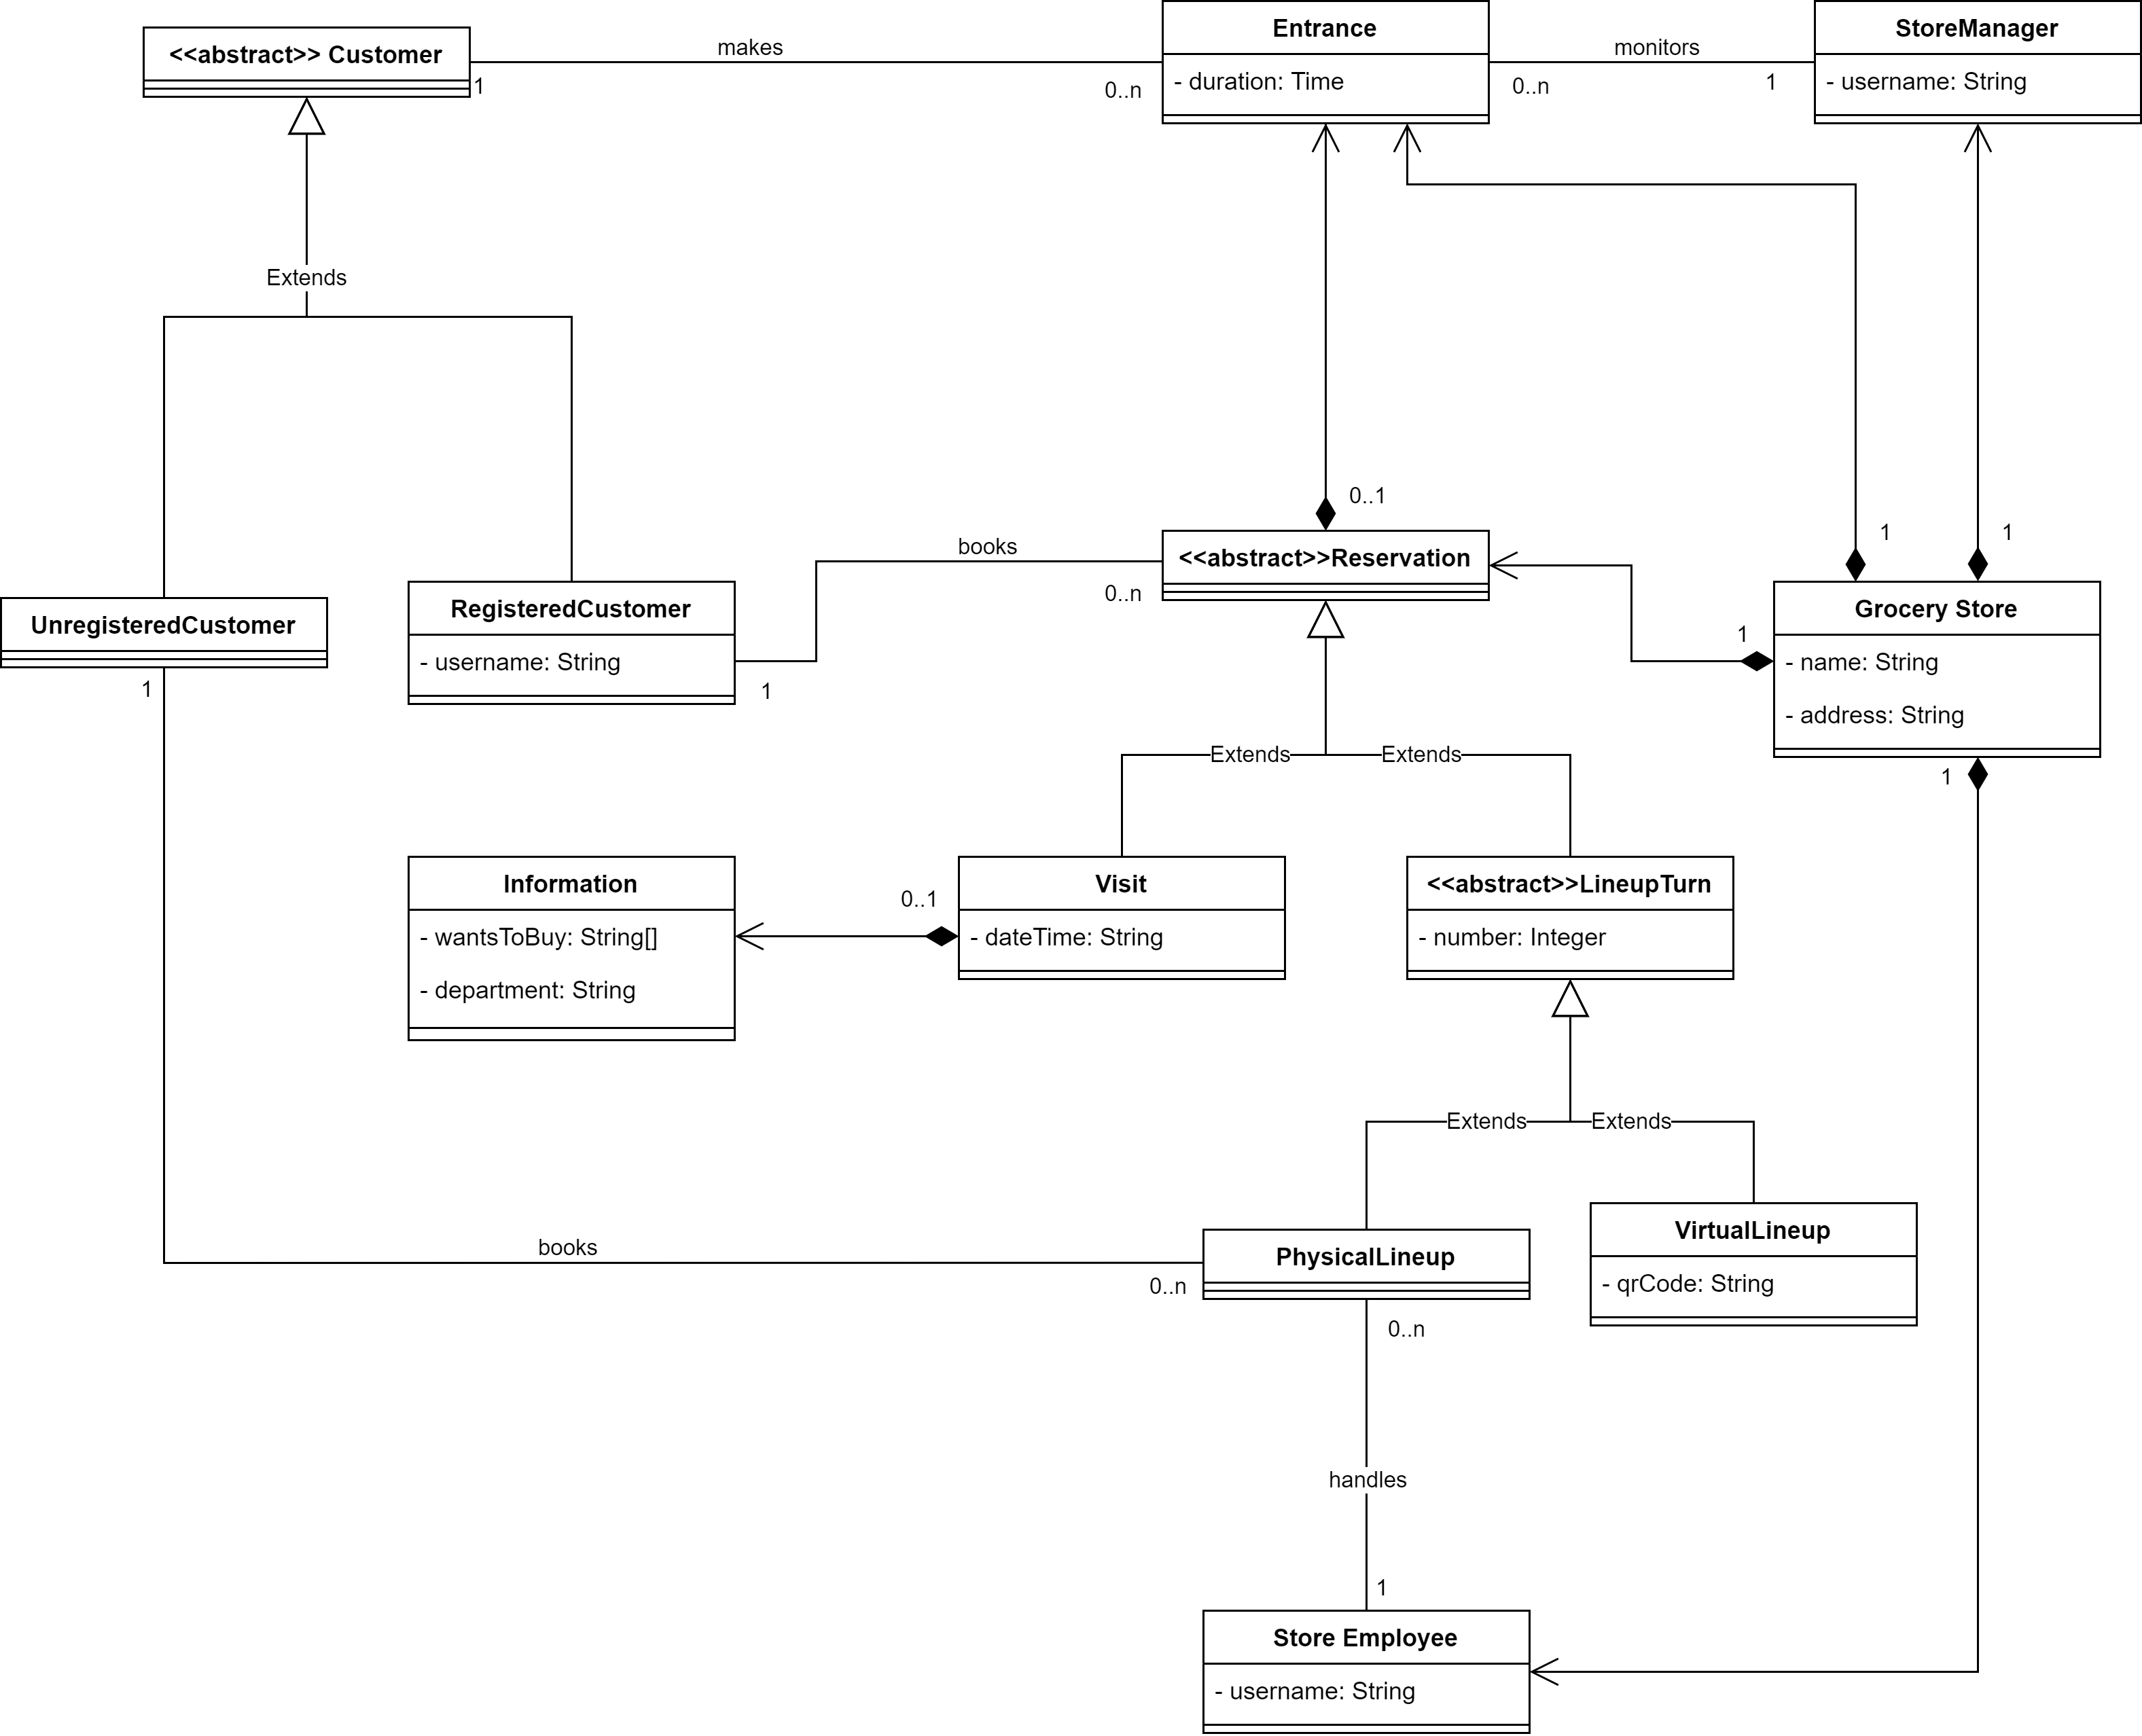
\includegraphics[width=\textwidth]{class_diagram.png}


\subsubsection{Dynamic Class Behaviour Models}
The below state diagrams shows some	critical aspects of	the	application, how the behaviour of these critical aspects is modeled and the evolution of their states.

\medskip
In the first state diagram, we model the behavior our system has to have when there is a new request to reserve a virtual lineup turn. Particular attention is paid to the possibility of generating a QR code and the management of waiting in the virtual lineup.

\medskip
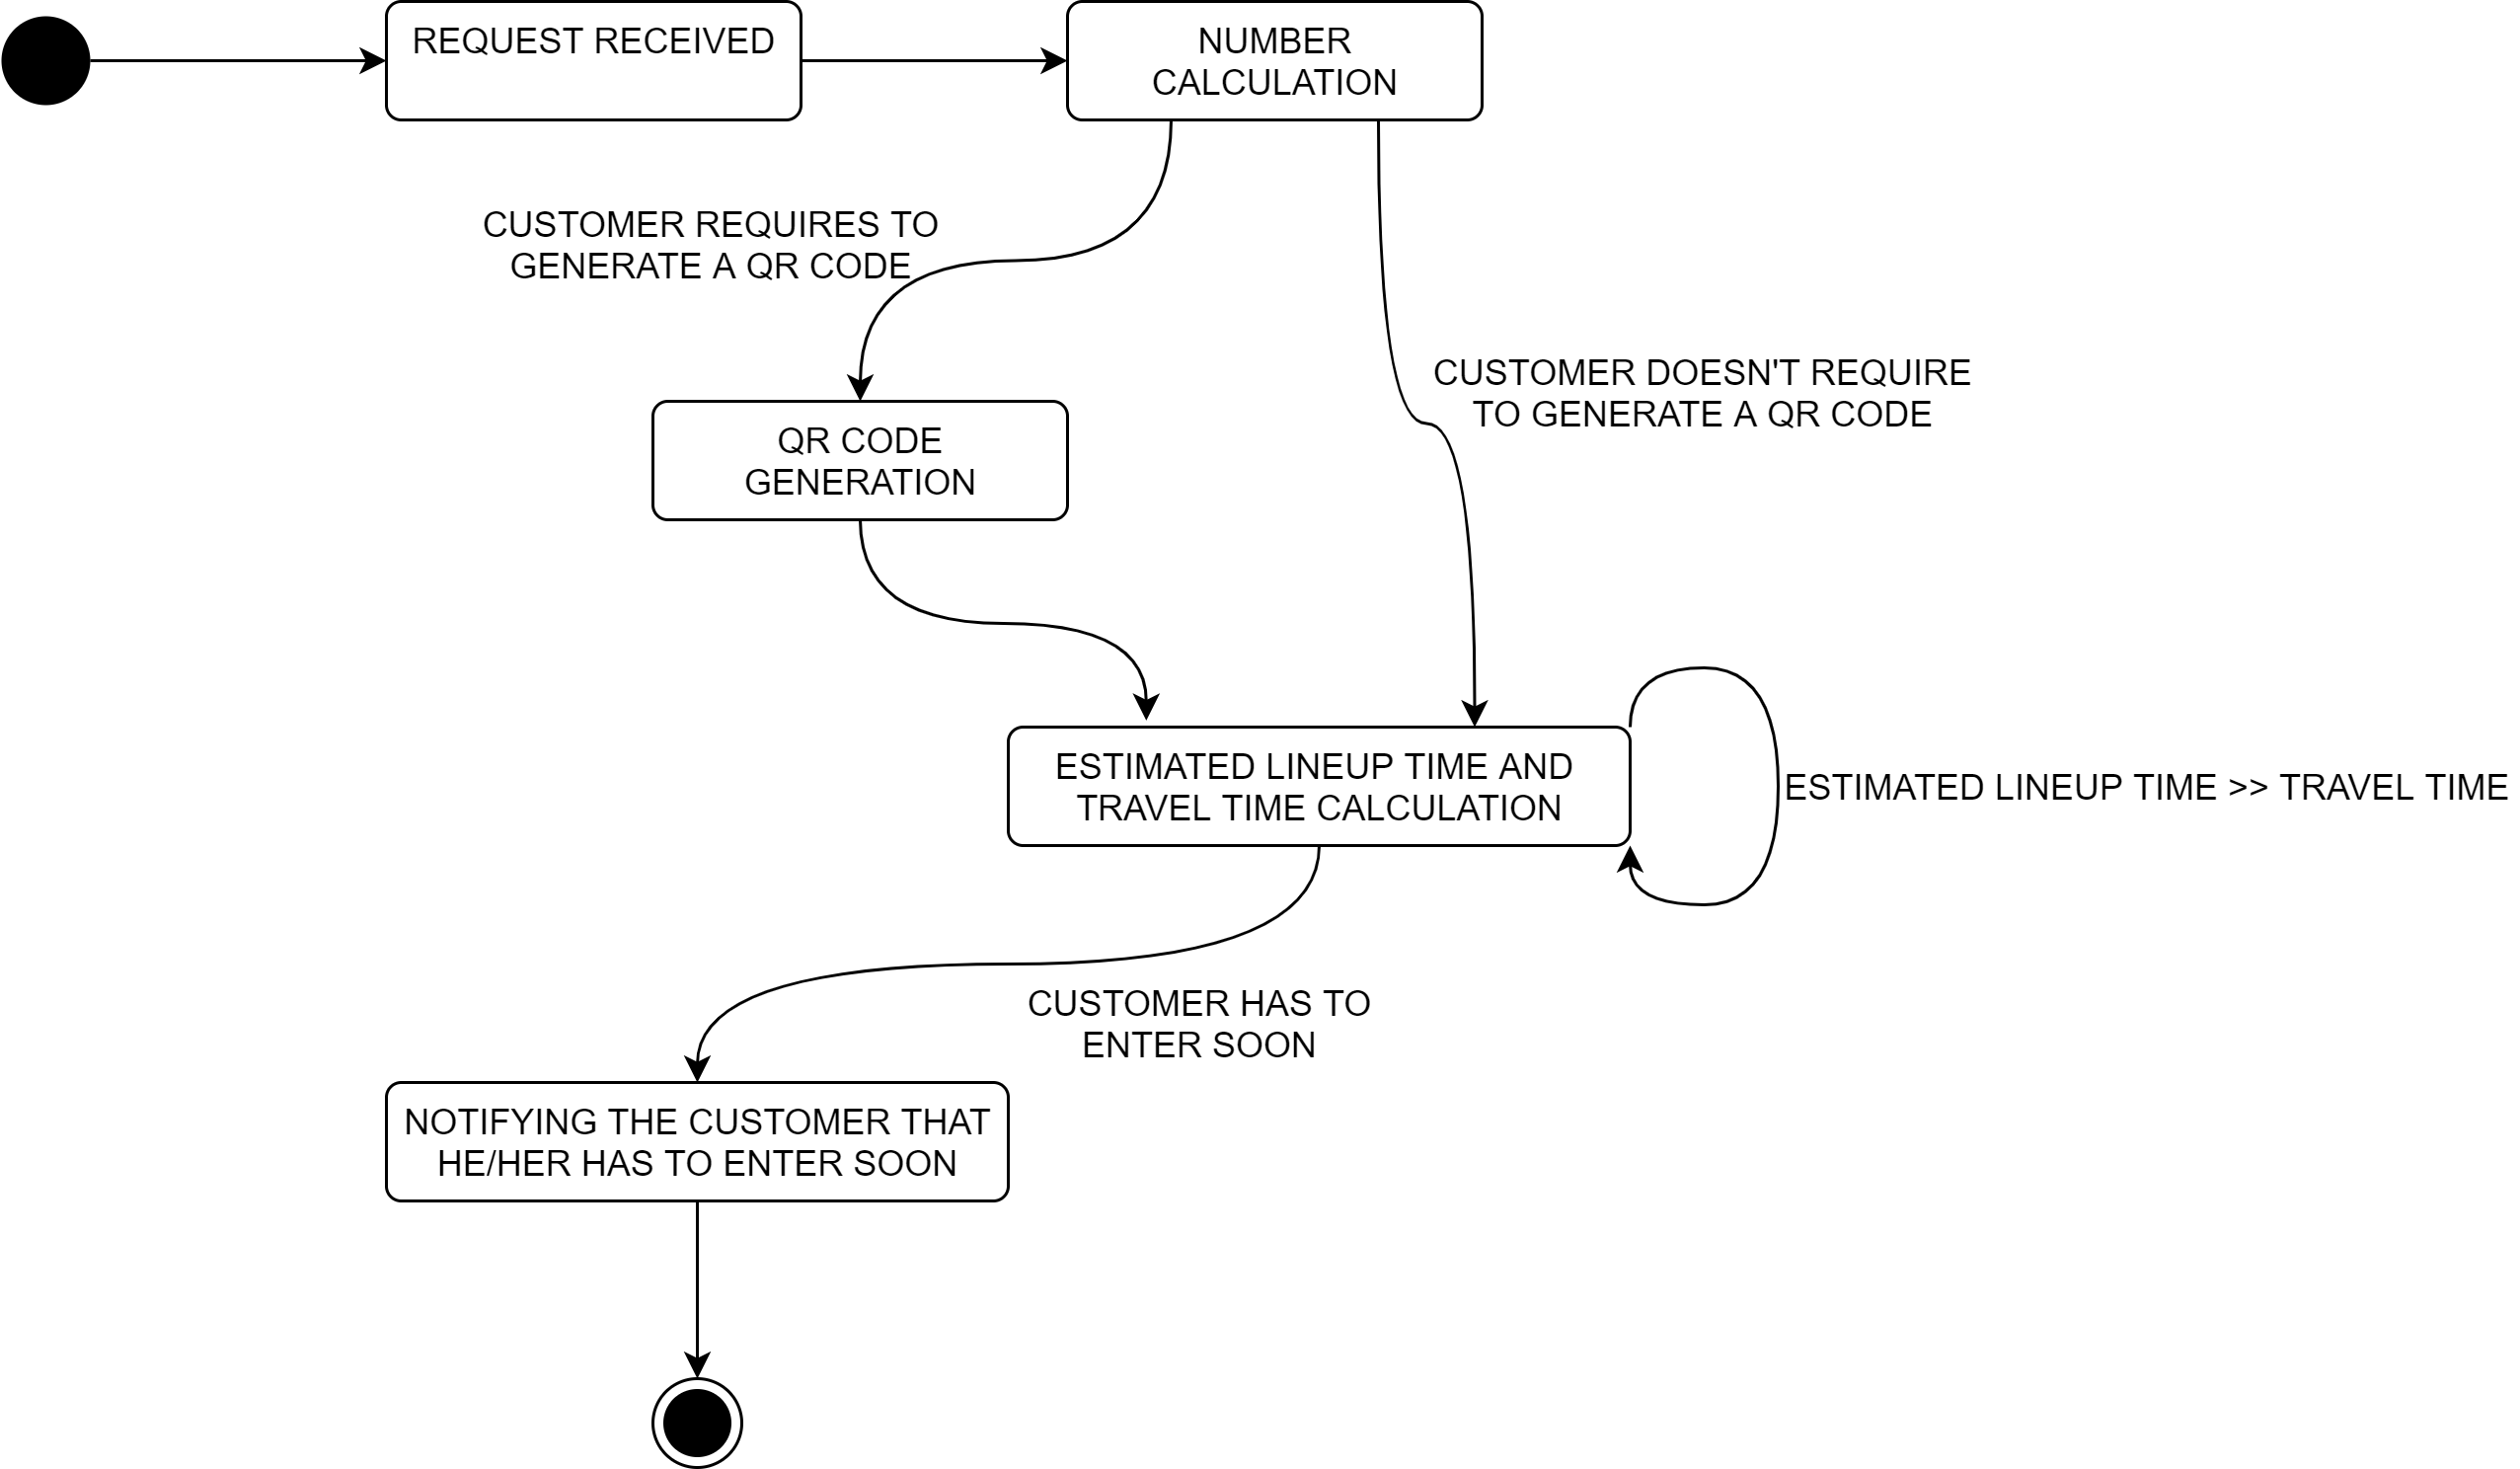
\includegraphics[width=\textwidth]{state_diagram1.png}

\medskip
In the second state diagram, we model the behavior our system has to have when a store employee notifies a new request to reserve a physical lineup turn. Attention is paid to the difference from the previous phenomenon. In this case, the system will limit itself to acquire the demand and to process it with the other demands (also virtual)

\medskip
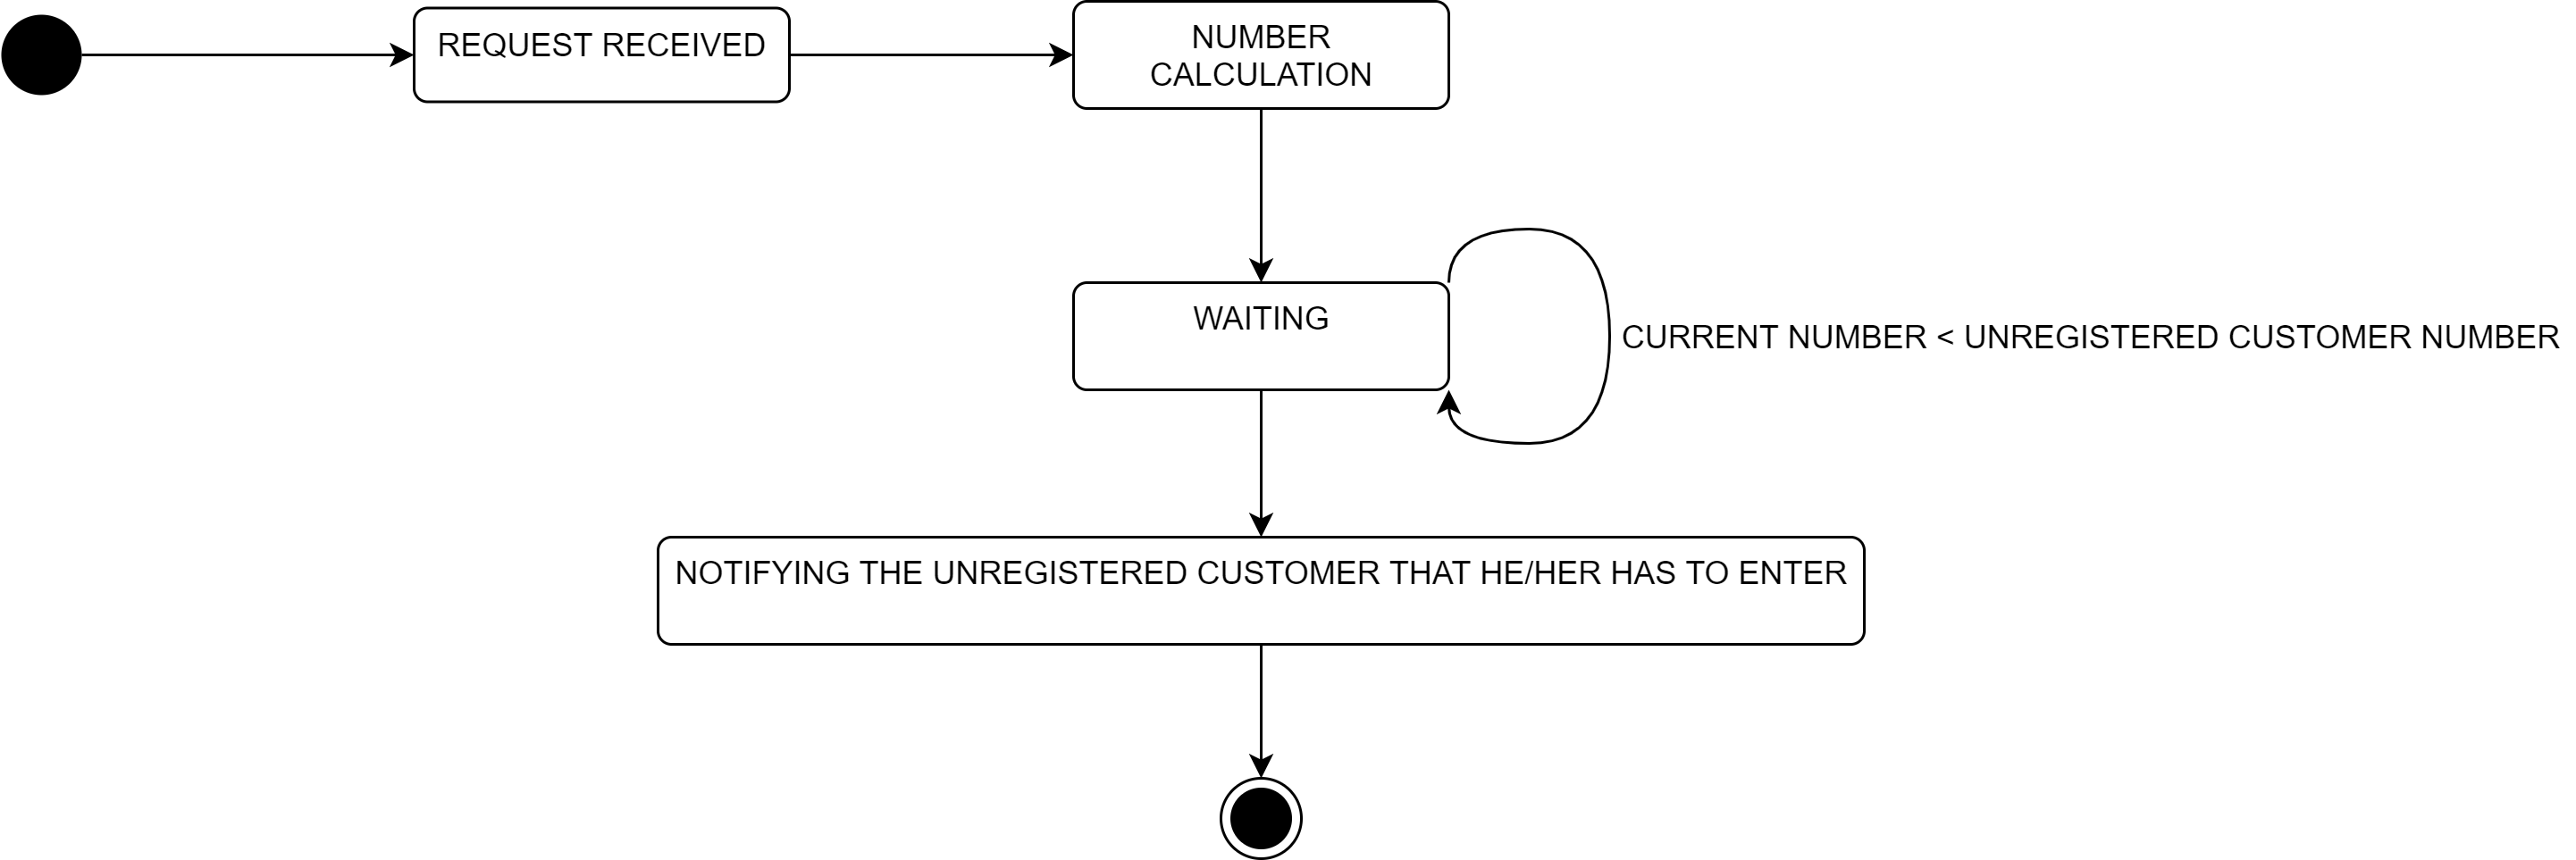
\includegraphics[width=\textwidth]{state_diagram2.png}

\medskip
In the third and last diagram, we model the behavior our system has to have when there is a new request for booking a visit. Attention is paid to the possibility of following various paths to reach the end of the request. These numerous paths are due to the optional insertion of information related to the visit (department, products to buy, and estimated time). Also, for long-term customers, the estimated time could be calculated by the system based on previous entries.

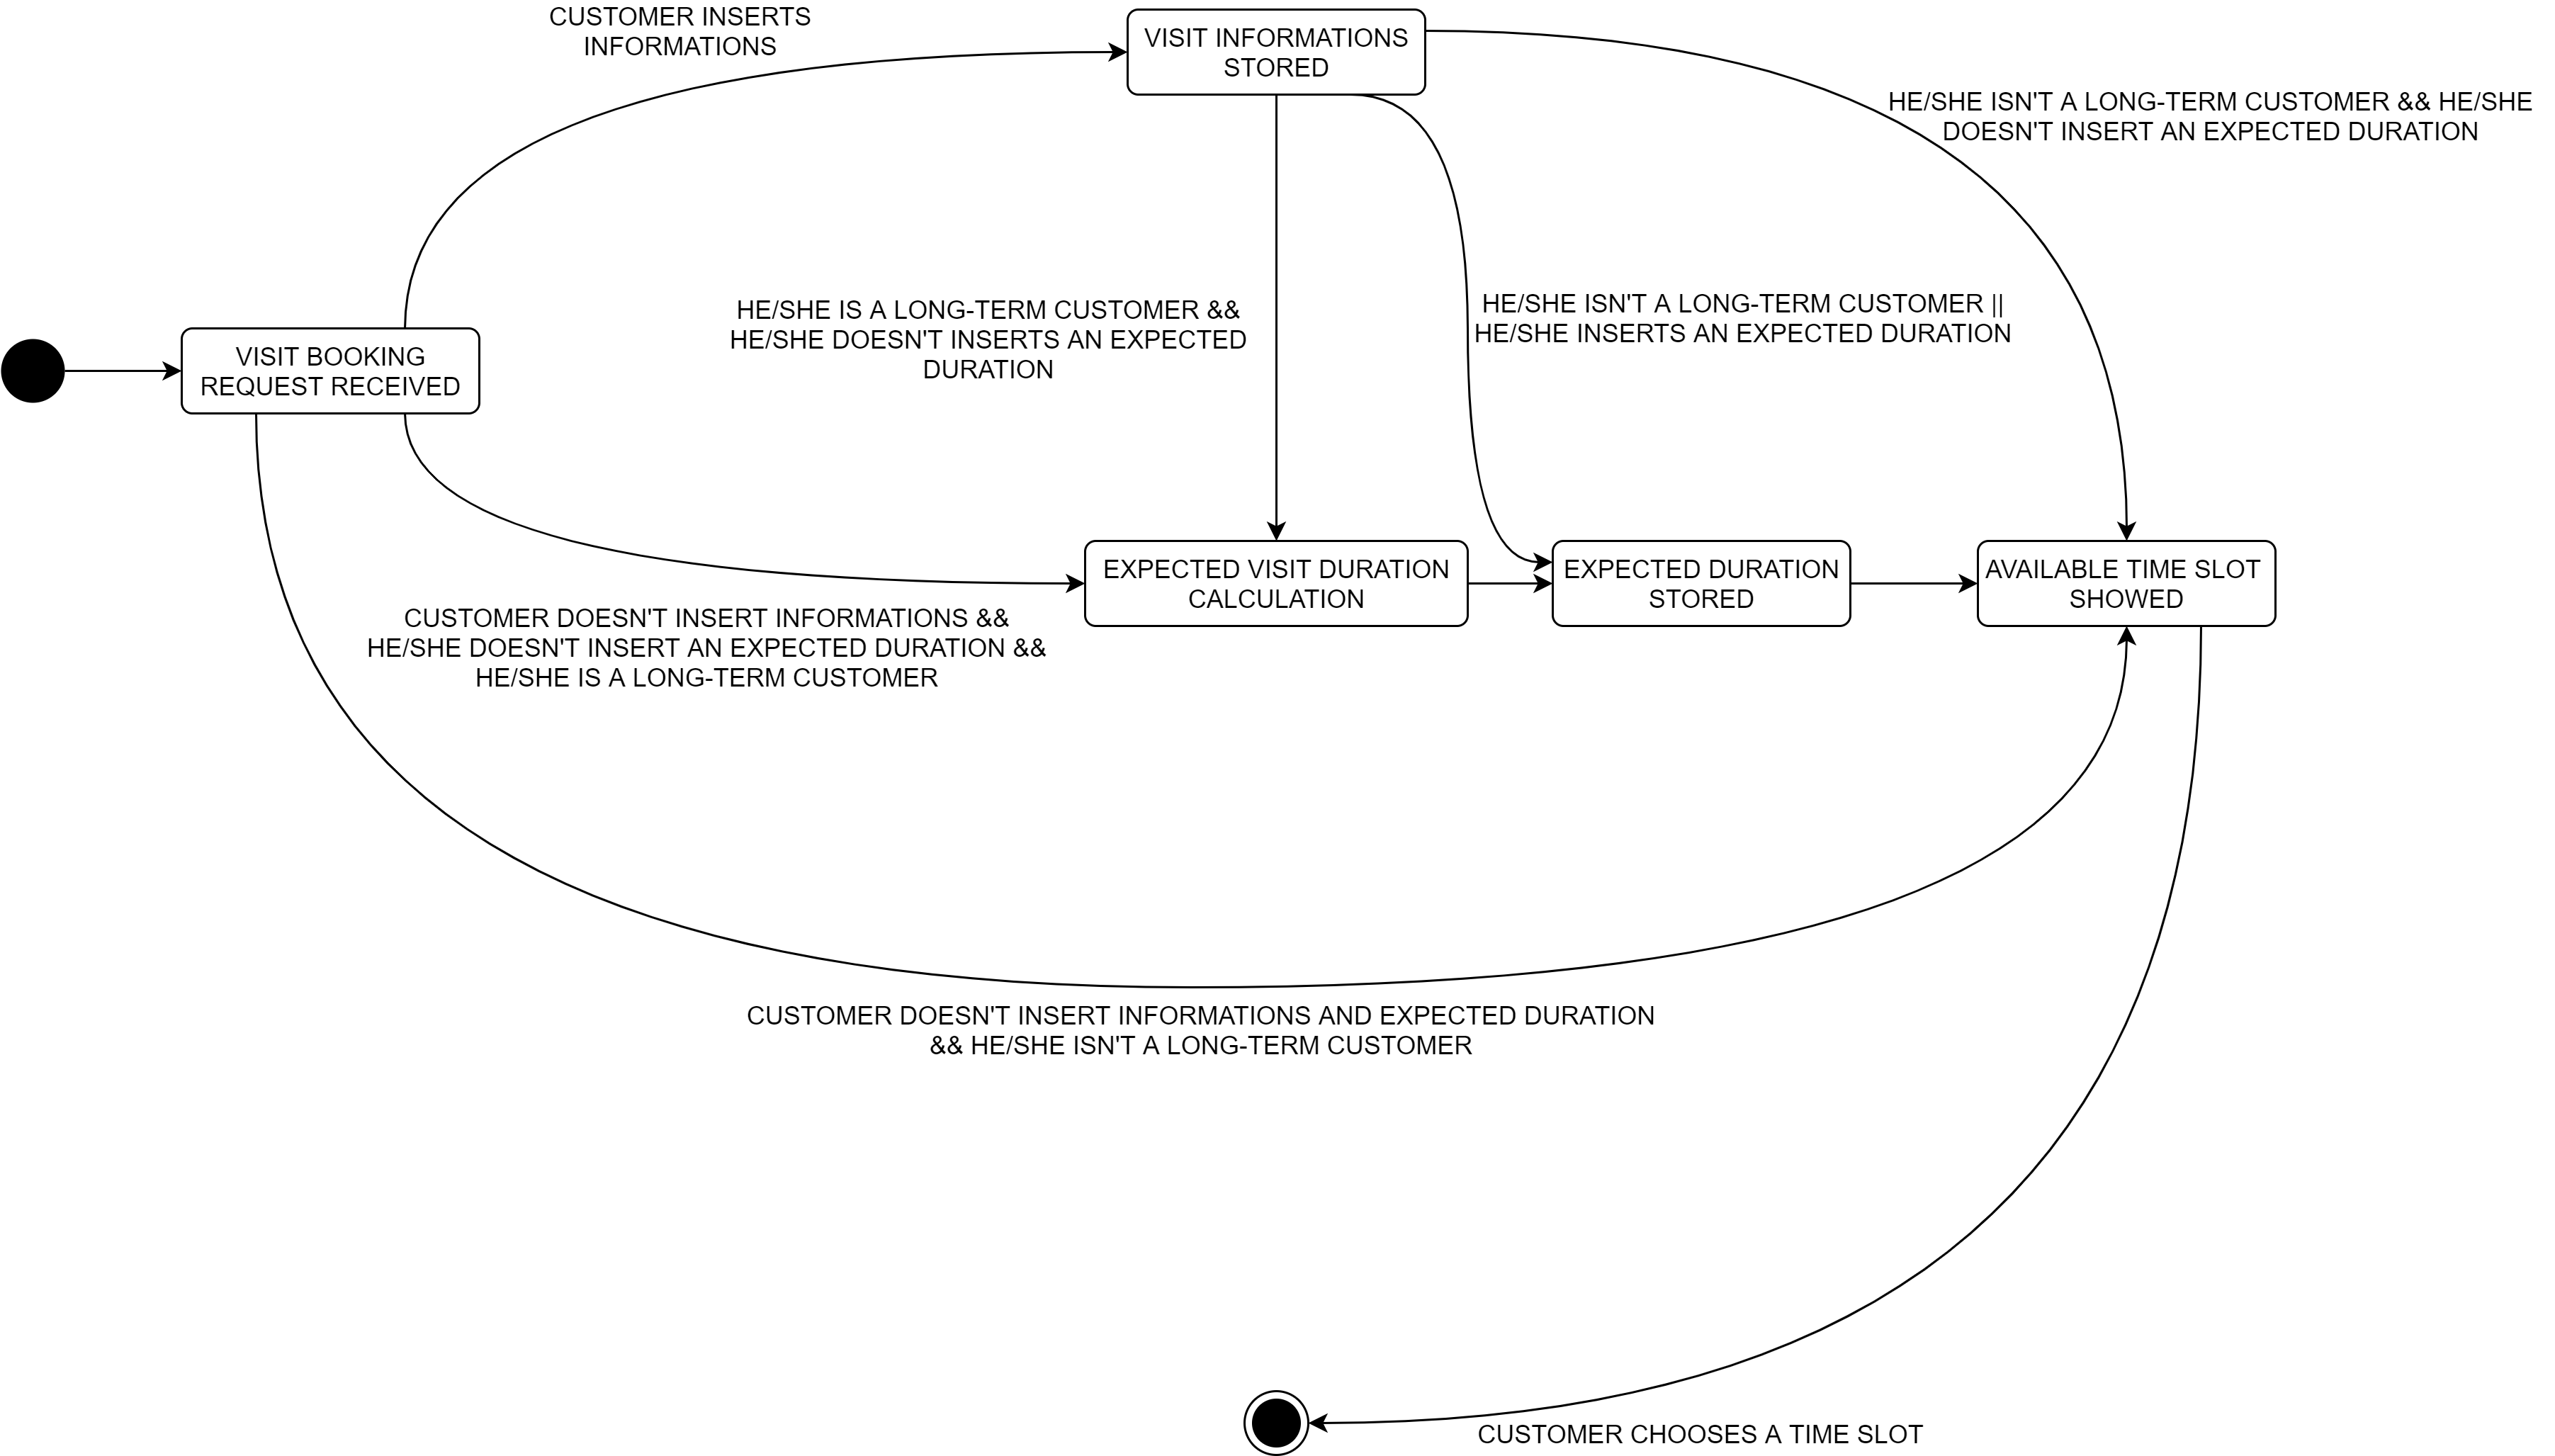
\includegraphics[width=\textwidth]{state_diagram3.png}